% !TeX root=../main.tex

\chapter{پاسخ سوالات سری اول}

% دستور زیر باعث عدم‌نمایش شماره صفحه در اولین صفحهٔ این فصل می‌شود.
%\thispagestyle{empty}
\section{ پاسخ سوال 1}

\subsection{بخش 1}

\subsubsection{قسمت یک}
برای حل این مسئله ی بهینه سازی، با استفاده از یک کد متلب ابتدا نابرابری های داده شده در یک نمودار دو بعدی ترسیم شده و ناحیه ی اشتراک حاصل از این خطوط  برای پاسخ های ممکن به دست می آید.

\begin{latin}
	\begin{lstlisting}[frame=single,style=Matlab-Pyglike]
		
% Solve pairs of equations symbolically for intersections
syms x1 x2

% Line equations:
eq1 = x1 + 2*x2 == 8;          % From x1 + 2*x2 = 8
eq2 = 3*x1 + 2*x2 == 12;       % From 3*x1 + 2*x2 = 12
eq3 = x1 + x2 == 4;            % From x1 + x2 = 4

% Solve intersections
% Intersection of eq1 and eq2
sol_1_2 = solve([eq1, eq2], [x1, x2]);

% Intersection of eq1 and eq3
sol_1_3 = solve([eq1, eq3], [x1, x2]);

% Intersection of eq2 and eq3
sol_2_3 = solve([eq2, eq3], [x1, x2]);

% Step 2: Identify intercepts with axes
% x1 intercepts and x2 intercepts
intercept_x1 = solve(eq1, x1);   % x1-intercept of x1 + 2*x2 = 8
intercept_x2 = solve(eq2, x1);   % x1-intercept of 3*x1 + 2*x2 = 12

% Boundary points on axes
boundary_points = [0, 8/2; 4, 0]; % Intersections with axes: (0, 8/2), (4, 0)

% Collect all intersection points
points = [
double([sol_1_2.x1, sol_1_2.x2]);  % Intersection of eq1 and eq2
double([sol_1_3.x1, sol_1_3.x2]);  % Intersection of eq1 and eq3
double([sol_2_3.x1, sol_2_3.x2]);  % Intersection of eq2 and eq3
boundary_points                     % Intersection with axes
];

% Step 3: Objective function
f = @(x1, x2) 5*x1 + 6*x2;

% Evaluate the objective function at each point
f_vals = arrayfun(@(i) f(points(i, 1), points(i, 2)), 1:size(points, 1));

% Find the minimum value and corresponding point
[min_val, min_idx] = min(f_vals);
optimal_point = points(min_idx, :);

% Display the results
fprintf('Intersection points and corresponding function values:\n');
for i = 1:size(points, 1)
fprintf('Point (x1 = %.2f, x2 = %.2f), f(x1, x2) = %.2f\n', points(i, 1), points(i, 2), f_vals(i));
end
fprintf('Optimal point: (x1 = %.2f, x2 = %.2f), Minimum f(x1, x2) = %.2f\n', optimal_point(1), optimal_point(2), min_val);

% Step 4: Plot the feasible region and the intersection points
figure; hold on;

% Plot the feasible region
contourf(X1, X2, feasible_region, [1 1], 'FaceColor', 'r', 'EdgeColor', 'none');

% Plot the lines representing the inequalities
plot(x1_vals, (8 - x1_vals)/2, 'b', 'LineWidth', 1.5);     % x1 + 2*x2 = 8
plot(x1_vals, (12 - 3*x1_vals)/2, 'g', 'LineWidth', 1.5);  % 3*x1 + 2*x2 = 12
plot(x1_vals, 4 - x1_vals, 'm', 'LineWidth', 1.5);         % x1 + x2 = 4

% Plot intersection points
plot(points(:, 1), points(:, 2), 'ko', 'MarkerFaceColor', 'y', 'MarkerSize', 5);

% Highlight the optimal point
plot(optimal_point(1), optimal_point(2), 'ro', 'MarkerFaceColor', 'r', 'MarkerSize', 10);

% Add labels and title
xlabel('x1');
ylabel('x2');
title('Feasible Region and Intersection Points');
grid on;
hold off;

xlim([0 ])
ylim([0.0 10])
		
	\end{lstlisting}
\end{latin}

% TODO: \usepackage{graphicx} required
\begin{figure}
	\centering
	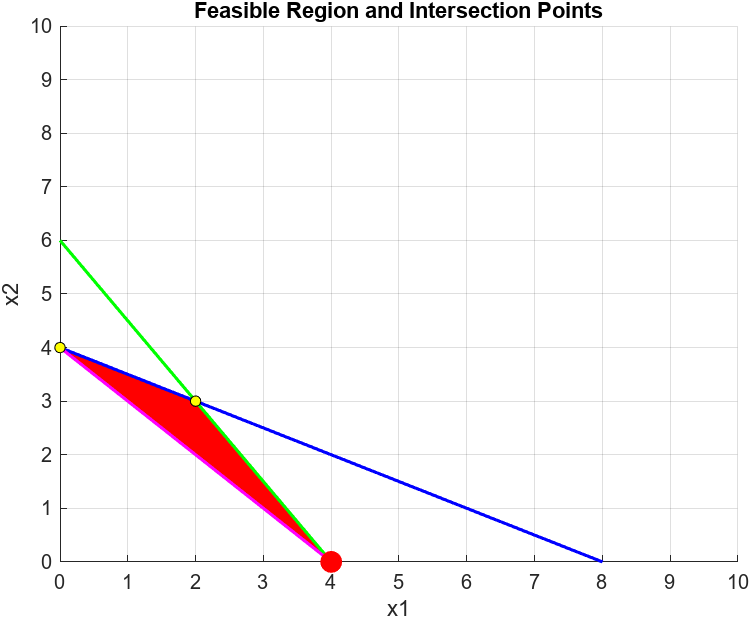
\includegraphics[width=1\linewidth]{../img/Q1_1}
	\caption{}
	\label{fig:q11}
\end{figure}

پاسخ بهینه برای معادله ی 
	\( f(x_1, x_2) = 5x_1 + 6x_2 \)
با جایگذاری مقادیر ممکن در معادله به دست می آید.
	
	\begin{itemize}
		\item \( (x_1 = 2.00, x_2 = 3.00) \), \( f(x_1, x_2) = 28.00 \)
		\item \( (x_1 = 0.00, x_2 = 4.00) \), \( f(x_1, x_2) = 24.00 \)
		\item \( (x_1 = 4.00, x_2 = 0.00) \), \( f(x_1, x_2) = 20.00 \)
		\item \( (x_1 = 0.00, x_2 = 4.00) \), \( f(x_1, x_2) = 24.00 \)
		\item \( (x_1 = 4.00, x_2 = 0.00) \), \( f(x_1, x_2) = 20.00 \)
	\end{itemize}
	
جواب بهینه برای این سوال برابر خواهد بود با:
	\[
	(x_1 = 4.00, x_2 = 0.00) , \quad f(x_1, x_2) = 20.00
	\]
\subsubsection{قسمت دو}
در این مرحله، با استفاده از ابزار های 
Yalmip
, 
CVX
مسئله ی بهینه سازی را حل می کنیم. در بخش اول، با استفاده از کد متلب زیر، محدودیت ها و تابع هزینه تعریف شده و در نهایت با اجرای کد، جواب های مورد نظر به دست می آید.

\begin{latin}
	\begin{lstlisting}[frame=single,style=Matlab-Pyglike]
		
yalmip('clear')
x1 = sdpvar(1,1)
x2 = sdpvar(1,1)

constraints = [x1<=8-2*x2 , 3*x1 + 2*x2<= 12, x1 + x2>=4 , x1>=0 , x2 >=0]

obj = 5*x1 + 6*x2

sol = optimize(constraints , obj)

if sol.problem ==0
val1 = value(x1)
val2 = value(x2)
objvalue = value(obj)
end
		
	\end{lstlisting}
\end{latin}

با استفاده از این کد، در نهایت جواب هایی مطابق با آنچه که به روش تحلیلی به دست آمد، حاصل می شود.

\[
(x_1 = 4.00, x_2 = 0.00) , \quad f(x_1, x_2) = 20.00
\]
در گام بعد، با استفاده از پکیج CVX، بار دیگر این مسئله حل می شود.


\begin{latin}
	\begin{lstlisting}[frame=single,style=Matlab-Pyglike]
		
cvx_begin

variables x1 x2

% Objective function
minimize(5*x1 + 6*x2)

% Subject to the constraints
subject to
x1 + 2*x2 <= 8
3*x1 + 2*x2 <= 12
x1 + x2 >= 4
x1 >= 0
x2 >= 0

cvx_end

% Display the results
x1_value = x1
x2_value = x2

		
	\end{lstlisting}
\end{latin}

\[
(x_1 = 4.00, x_2 = 0) , \quad f(x_1, x_2) = 20.00
\]

مشاهده می شود که با استفاده از این روش نیز، پاسخ مشابهی به دست می آید.

\subsection{بخش 2}
در این بخش، مشابه آنچه که در بخش پیشین انجام شد، ابتدا به روش تحلیلی و با رسم ناحیه ی نقاط امکان پذیری، نقاط بهینه تشخیص داده می شوند.
در کد متلب زیر، با تعیین معادلات مربوط به محدودیت ها، و محاسبه ی نقاط تقاطع خطوط، پاسخ بهینه به دست آمده و نمایش داده شده است.

\begin{latin}
	\begin{lstlisting}[frame=single,style=Matlab-Pyglike]
		
% Clear previous variables
clear; clc;

% Step 1: Define symbolic variables
syms x1 x2;

% Step 2: Define the constraints
% Lines based on constraints
eq1 = x1 + x2 == -20;  % From x1 + x2 = -20
eq2 = x1 + x2 == 5;    % From x1 + x2 = 5

% Step 3: Solve intersections
% Intersection of eq1 and eq2
sol_1_2 = solve([eq1, eq2], [x1, x2]);

% Define boundaries for x1 and x2
boundary_x1 = [-5, 5];  % x1 boundaries
boundary_x2 = [-1, 5];  % x2 boundaries

% Collect boundary points based on the constraints
boundary_points = [
-5, -1;   % Bottom left corner
-5, 5;    % Top left corner
5, -1;    % Bottom right corner
0, 5;     % Top right corner
5,0
];

% Collect all intersection points (if valid)
points = [
double([sol_1_2.x1, sol_1_2.x2]);  % Intersection of eq1 and eq2
boundary_points                     % Intersections with axes
];

% Step 4: Define the objective function
f = @(x1, x2) abs(x1 - 5) + abs(x2 - 5);

% Step 5: Evaluate the objective function at each point
% Filter valid points based on constraints
valid_points = points((points(:,1) >= boundary_x1(1)) & (points(:,1) <= boundary_x1(2)) & ...
(points(:,2) >= boundary_x2(1)) & (points(:,2) <= boundary_x2(2)), :);

f_vals = arrayfun(@(i) f(valid_points(i, 1), valid_points(i, 2)), 1:size(valid_points, 1));

% Step 6: Find the minimum value and corresponding point
[min_val, min_idx] = min(f_vals);
optimal_point = valid_points(min_idx, :);

% Display the results
fprintf('Valid points and corresponding function values:\n');
for i = 1:size(valid_points, 1)
fprintf('Point (x1 = %.2f, x2 = %.2f), f(x1, x2) = %.2f\n', valid_points(i, 1), valid_points(i, 2), f_vals(i));
end
fprintf('Optimal point: (x1 = %.2f, x2 = %.2f), Minimum f(x1, x2) = %.2f\n', optimal_point(1), optimal_point(2), min_val);

% Step 7: Plot the feasible region and the intersection points
figure; hold on;

% Create a grid for plotting feasible region
[x1_vals, x2_vals] = meshgrid(-5:0.1:5, -1:0.1:5);
feasible_region = (x1_vals + x2_vals >= -20) & (x1_vals + x2_vals <= 5 & ...
(-5 <= x1_vals) & (x1_vals <= 5) & (-1 <= x2_vals) & (x2_vals <= 5));

% Plot the feasible region
contourf(x1_vals, x2_vals, feasible_region, [1 1], 'FaceColor', 'r', 'EdgeColor', 'none');

% Plot the constraint lines
plot(x1_vals, -20 - x1_vals, 'k', 'LineWidth', 1.5); % x1 + x2 = -20
plot(x1_vals, 5 - x1_vals, 'k', 'LineWidth', 1.5);   % x1 + x2 = 5

% Plot intersection points
plot(valid_points(:, 1), valid_points(:, 2), 'ko', 'MarkerFaceColor', 'y', 'MarkerSize', 8);

% Highlight the optimal point
plot(optimal_point(1), optimal_point(2), 'ro', 'MarkerFaceColor', 'g', 'MarkerSize', 10);

% Add labels and title
xlabel('x1');
ylabel('x2');
title('Feasible Region and Intersection Points');
grid on;
hold off;

% Set axis limits
xlim([-6 6]);
ylim([-2 6]);

	\end{lstlisting}
\end{latin}


% TODO: \usepackage{graphicx} required
\begin{figure}[H]
	\centering
	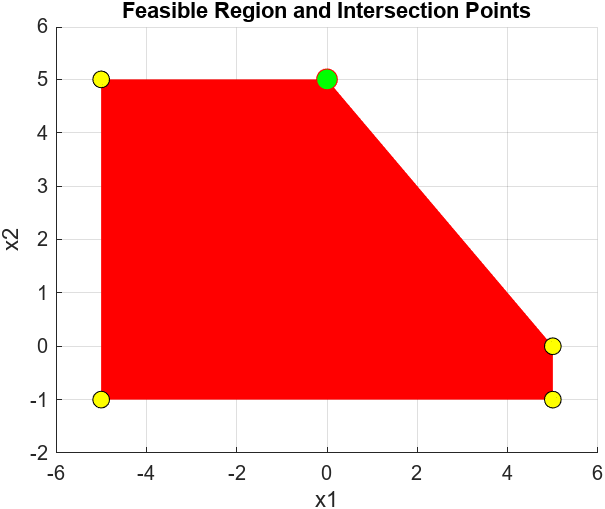
\includegraphics[width=1\linewidth]{../img/Q2_1}
	\caption{}
	\label{fig:q21}
\end{figure}

پاسخ بهینه برای تابع هزینه، با جایگذاری نقاط در آن و انتخاب مقدار کمینه به دست می آید.

\[
(x_1 = 0.00, x_2 = 5) , \quad f(x_1, x_2) = 5
\]

در قسمت بعد، بار اول با استفاده از پکیج 
Yalmip
و بار دیگر با استفاده از پکیج 
CVX
مسئله ی بهینه سازی را حل می کنیم.

Yalmip:

\begin{latin}
	\begin{lstlisting}[frame=single,style=Matlab-Pyglike]
		
% Clear previous variables
clear; clc;

% Step 1: Define the variables
x1 = sdpvar(1,1);  % Decision variable x1
x2 = sdpvar(1,1);  % Decision variable x2

% Step 2: Define the objective function
objective = abs(x1 - 5) + abs(x2 - 5);

% Step 3: Define the constraints
constraints = [
-5 <= x1 <= 5,      % Constraint for x1
-1 <= x2 <= 5,      % Constraint for x2
-20 <= x1 + x2 <= 5 % Constraint for the sum of x1 and x2
];

% Step 4: Solve the optimization problem
options = sdpsettings('verbose', 1);  % Set verbosity to see solver output
sol = optimize(constraints, objective, options);

% Step 5: Check the results
if sol.problem == 0
% If no error, display the results
optimal_x1 = value(x1);
optimal_x2 = value(x2);
optimal_value = value(objective);

fprintf('Optimal point: (x1 = %.2f, x2 = %.2f), Minimum f(x1, x2) = %.2f\n', ...
optimal_x1, optimal_x2, optimal_value);
else
% If there was an error, display the error message
disp('Solver encountered an issue:');
disp(sol.info);
end

		
	\end{lstlisting}
\end{latin}

\[
(x_1 = 5.00, x_2 = 0) , \quad f(x_1, x_2) = 5.00
\]

CVX:

\begin{latin}
	\begin{lstlisting}[frame=single,style=Matlab-Pyglike]
		
% Clear previous variables
clear; clc;

% Step 1: Start CVX
cvx_begin

% Step 2: Define the variables
variables x1 x2;  % Decision variables x1 and x2

% Step 3: Define the objective function
minimize(abs(x1 - 5) + abs(x2 - 5));

% Step 4: Define the constraints
subject to
-5 <= x1 <= 5;      % Constraint for x1
-1 <= x2 <= 5;      % Constraint for x2
-20 <= x1 + x2 <= 5; % Constraint for the sum of x1 and x2

cvx_end

% Step 5: Display the results
fprintf('Optimal point: (x1 = %.2f, x2 = %.2f), Minimum f(x1, x2) = %.2f\n', x1, x2, abs(x1 - 5) + abs(x2 - 5));
		
	\end{lstlisting}
\end{latin}

\[
(x_1 = 2.32, x_2 = 2.68) , \quad f(x_1, x_2) = 5.00
\]

مشاهده می شود که پاسخ به دست آمده توسط روش 
CVX
با مقدار به دست آمده از 
Yalmip
تفاوت دارد. در حالی که جواب CVX از نقاط گوشه نیست، اما پاسخ درستی برای مسئله ی بهینه سازی است و می تواند به عنوان نقطه ی بهینه انتخاب شود.
\section{پاسخ سوال 2}
در این سوال، مانند قسمت قبل باید ابتدا تابع هزینه و سپس محدودیت ها مشخص شوند. تفاوت این سوال، به دلیل تغییر در نحوه ی بیان محدودیت ها است که در غالب ماتریس داده شده است. بنابراین، با تبدیل آن به فرم معادلات خطی خواهیم داشت:

\begin{align*}
	x_1 - 2x_2 &\geq -2, \\
	-x_1 - 2x_2 &\geq -6, \\
	-x_1 + x_2 &\geq -2, \\
	x_1 &\geq 0, \\
	x_2 &\geq 0.
\end{align*}

برای حل این سوال و استفاده از پکیج
 yalmip
  و
 cvx
  در کدهای متلب که در ادامه آمده است، مسئله ی بهینه سازی را حل می کنیم.

\textbf{Yalmip:}
\begin{latin}
	\begin{lstlisting}[frame=single,style=Matlab-Pyglike]
		
yalmip('clear')

% Define variables
x1 = sdpvar(1,1);
x2 = sdpvar(1,1);

% Define objective function
objective = (x1 - 1)^2 + (x2 - 2.5)^2;

% Define constraints
constraints = [x1 - 2*x2 >= -2, ...
-x1 - 2*x2 >= -6, ...
-x1 + x2 >= -2, ...
x1 >= 0, x2 >= 0];

% Solve problem
optimize(constraints, objective)

% Display solution
solution_x1 = value(x1)
solution_x2 = value(x2)
solution_obj = value(objective)

disp(['Optimal x1: ', num2str(solution_x1)])
disp(['Optimal x2: ', num2str(solution_x2)])
disp(['Optimal objective value: ', num2str(solution_obj)])
	\end{lstlisting}
\end{latin}

\[
(x_1 = 1.4, x_2 = 1.7) , \quad f(x_1, x_2) = 0.8
\]

\textbf{CVX:}

\begin{latin}
	\begin{lstlisting}[frame=single,style=Matlab-Pyglike]
		
cvx_begin
variables x1 x2
% Objective function
minimize((x1 - 1)^2 + (x2 - 2.5)^2)

% Constraints
subject to
x1 - 2*x2 >= -2
-x1 - 2*x2 >= -6
-x1 + x2 >= -2
x1 >= 0
x2 >= 0
cvx_end

% Display solution
disp(['Optimal x1: ', num2str(x1)])
disp(['Optimal x2: ', num2str(x2)])
disp(['Optimal objective value: ', num2str(cvx_optval)])
	\end{lstlisting}
\end{latin}

\[
(x_1 = 1.4, x_2 = 1.7) , \quad f(x_1, x_2) = 0.8
\]

مشاهده می شود که با استفاده از هر دو روش، نتایج یکسانی به دست می آید.

\section{پاسخ سوال 3}

با توجه به معادله ی داده شده در این سوال، مشاهده می شود که بر خلاف مسائل پیشین، در این مثال نواحی مرزی تعیین نشده است و یک مثال بهینه سازی نامحدود است. پیش از انجام محاسبات به روش تحلیلی و پیدا کردن نقطه ی کمینه، ابتدا با رسم نمودار معادله، درکی از رفتار آن به دست می آوریم.



\begin{figure}[H]
	\centering
	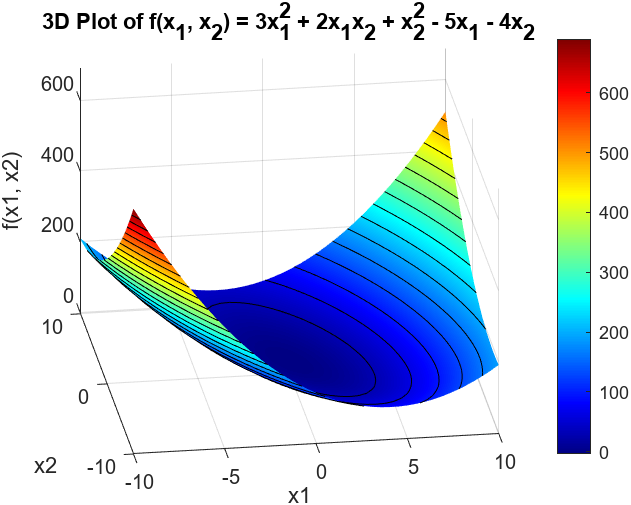
\includegraphics[width=1\linewidth]{../img/Q3_1}
	\caption{}
	\label{fig:q31}
\end{figure}

همان طور که بیان شد، مشاهده می شود که می توان یک نقطه ی کمینه برای این مثال پیدا کرد.

با در اختیار داشتن معادله که در این قسمت مجددا آورده شده است، لازم است مشتق آن نسبت به x1 و x2 گرفته شده و با برابر صفر قرار دادن هر یک از آنها، مقادیر مورد نظر به دست آید. در ادامه ی این بخش، به شرح این فرایند خواهیم پرداخت.

\[
f(x_1, x_2) = 3x_1^2 + 2x_1x_2 + x_2^2 - 5x_1 - 4x_2
\]


مشتق اول عبارت فوق برابر است با:

\[
\nabla f(x_1, x_2) = \left[ \frac{\partial f}{\partial x_1}, \frac{\partial f}{\partial x_2} \right] = \left[ 6x_1 + 2x_2 - 5, 2x_1 + 2x_2 - 4 \right]
\]

با برابر صفر قرار دادن مشتقات خواهیم داشت:

\[
6x_1 + 2x_2 - 5 = 0
\]
\[
2x_1 + 2x_2 - 4 = 0
\]


از حل این معادله، به دست می آید:

\[
x_1 = \frac{1}{4}, \quad
x_2 = \frac{7}{4}
\]

با محاسبه ی ماتریس مشتق مرتبه دوم و بررسی المان های ماتریس هسین، می توانیم مشخص کنیم که نقاط به دست آمده، از چه نوع اکسترمم هستند. برای این کار خواهیم داشت:

\[
H = \begin{bmatrix}
	\frac{\partial^2 f}{\partial x_1^2} & \frac{\partial^2 f}{\partial x_1 \partial x_2} \\
	\frac{\partial^2 f}{\partial x_2 \partial x_1} & \frac{\partial^2 f}{\partial x_2^2}
\end{bmatrix} = \begin{bmatrix}
	6 & 2 \\
	2 & 2
\end{bmatrix}
\]

از آنجا که ماتریس هسین به دست آمده مثبت معین است، بنابراین نقاط به دست آمده، معادل نقطه ی مینیمم می باشند.

در مرحله ی بعد، با استفاده از پکیج های بهینه سازی، به حل این مسئله خواهیم پرداخت.

\textbf{Yalmip:}
\begin{latin}
	\begin{lstlisting}[frame=single,style=Matlab-Pyglike]
		
% Clear workspace
clear; clc;

% Define variables
x = sdpvar(2,1);

% Define the objective function
f = 3*x(1)^2 + 2*x(1)*x(2) + x(2)^2 - 5*x(1) - 4*x(2);

% Set up the optimization problem
optimize([], f);

% Display the results
optimal_x = value(x);
optimal_fval = value(f);

fprintf('Optimal x1 = %.4f, Optimal x2 = %.4f\n', optimal_x(1), optimal_x(2));
fprintf('Minimum value of the function: %.4f\n', optimal_fval);
	\end{lstlisting}
\end{latin}

\[
(x_1 = 0.25, x_2 = 1.75) , \quad f(x_1, x_2) = -4.1250
\]

\textbf{CVX:}

\begin{latin}
	\begin{lstlisting}[frame=single,style=Matlab-Pyglike]
		
% Clear workspace and previous CVX problem
clear; clc;
cvx_clear;

% Use CVX for solving the optimization problem
cvx_begin
variables x1 x2
% Define the objective function
f = 3*x1^2 + 2*x1*x2 + x2^2 - 5*x1 - 4*x2;

% Use 'minimize' function for the objective
minimize(f)
cvx_end

% Display the results
fprintf('Optimal x1 = %.4f, Optimal x2 = %.4f\n', x1, x2);
fprintf('Minimum value of the function: %.4f\n', f);

	\end{lstlisting}
\end{latin}

با اجرای کد CVX، مشاهده می شود که این پکیج قادر به حل این مسئله نیست و با خطا روبه رو می شود.

در بخش بعد، برای پیدا کردن نقطه ی ماکسیمم، باید علامت منفی در تابع ضرب شود. بنابراین، مطاب قآنچه که در نمودار نمایش داده شده برای این معادله دیده شد و همچنین با توجه به ماهیت معادله که محدب و نامحدود است، می توان نتیجه گرفت که این معادله مقدار بیشینه ای ندارد و یا مقدار آن برابر بی نهایت است. 
در محاسبه ی تحلیلی این قضیه، مشاهده کردیم که تنها یک جواب به دست آمد و با بررسی ماتریس هسین دیدیم که این مقدار، مربوط به مینیمم تابع است. بنابراین، به روش تحلیلی می توان نتیجه گرفت که این معادله مقدار ماکسیمم ندارد.

در ادامه با استفاده از پکیج های Yalmip و CVX، صحت این موضوع را بررسی می کنیم.

\textbf{Yalmip:}
\begin{latin}
	\begin{lstlisting}[frame=single,style=Matlab-Pyglike]
% Clear workspace
clear; clc;

% Define variables
x = sdpvar(2,1);

% Define the objective function (negated for maximization)
f = -(3*x(1)^2 + 2*x(1)*x(2) + x(2)^2 - 5*x(1) - 4*x(2));

% Set up the optimization problem
optimize([], f);

% Display the results (negated back)
optimal_x = value(x);
optimal_fval = -value(f); % negate the function value back

fprintf('Optimal x1 = %.4f, Optimal x2 = %.4f\n', optimal_x(1), optimal_x(2));
fprintf('Maximum value of the function: %.4f\n', optimal_fval);
	\end{lstlisting}
\end{latin}

\[
(x_1 = -243236479749.1021, x_2 = -130439567620.7782) 
\]

\[
\quad f(x_1, x_2) = 257961758541185663631360.0000
\]

مشاهده می شود که مقادیر گزارش شده به دلیل محدودیت در انجام محاسبات است و بیشتری

\textbf{CVX:}
\begin{latin}
	\begin{lstlisting}[frame=single,style=Matlab-Pyglike]
% Clear workspace
clear; clc;

% Use CVX for solving the maximization problem
cvx_begin
variables x1 x2
% Define the objective function (negated for maximization)
f = -(3*x1^2 + 2*x1*x2 + x2^2 - 5*x1 - 4*x2);
minimize(f)
cvx_end

% Display the results (negated back)
fprintf('Optimal x1 = %.4f, Optimal x2 = %.4f\n', x1, x2);
fprintf('Maximum value of the function: %.4f\n', -f); % negate the function value back

	\end{lstlisting}
\end{latin}

مجددا مشاهده می شود که CVX نمی تواند این مسئله را حل کند.

\section{پاسخ سوال 4}
 
 برای حل این سوال، با بررسی تابع داده شده در می یابیم که به دلیل وجود ریشه چهارم در این عبارت، مقعر است. بنابراین، می توانیم اطمینان داشته باشیم که استفاده از پکیج های Yalmip و CVX قادر به حل این مسئله نخواهند بود. در ادامه، به اجرا و بررسی عملکرد این شبکه ها خواهیم پرداخت.
 
 \textbf{Yalmip:}
 \begin{latin}
 	\begin{lstlisting}[frame=single,style=Matlab-Pyglike]
% Clear workspace
clear; clc;

% Define variables
x1 = sdpvar(1,1);
x2 = sdpvar(1,1);

% Define the objective function
obj = sqrt(sqrt((x1 - x2^2)^2 + 0.02)) + 0.01*x2^2;

% Define any constraints (if applicable)
constraints = [];

% Set options for solver
options = sdpsettings('solver', 'fmincon', 'verbose', 1);

% Solve the problem
sol = optimize(constraints, obj, options);

% Check if the solution was successful
if sol.problem == 0
% Display the results
disp('Optimal solution found:');
disp('x1 =');
disp(value(x1));
disp('x2 =');
disp(value(x2));
disp('Objective value =');
disp(value(obj));
else
disp('Failed to find a solution');
disp(sol.info);
end
 		
 	\end{lstlisting}
 \end{latin}
 
  \textbf{CVX:}
 \begin{latin}
 	\begin{lstlisting}[frame=single,style=Matlab-Pyglike]
% Clear workspace
clear; clc;

% CVX optimization
cvx_begin
variables x1 x2
% Define the objective function
minimize( sqrt(sqrt((x1 - x2^2)^2 + 0.02)) + 0.01*x2^2 )
cvx_end

% Display the results
disp('Optimal solution found:');
disp('x1 =');
disp(x1);
disp('x2 =');
disp(x2);
disp('Objective value =');
disp(cvx_optval);
 	\end{lstlisting}
 \end{latin}
 
 مطابق آنچه که انتظار داشتیم، اجرای هیچ یک از این دو روش نتایجی به دست نمی دهد. علت دیگری که مانع اجرای صحیح این شبکه ها می شود، بنابراین، با استفاده از الگوریتم های پیشرفته تر نظیر الگوریتم ژنتیک، تابع را بهینه سازی می کنیم.
 
   \textbf{GA:}
 \begin{latin}
 	\begin{lstlisting}[frame=single,style=Matlab-Pyglike]
% Clear workspace
clear; clc;

% Define the objective function
obj = @(x) sqrt(sqrt((x(1) - x(2)^2)^2 + 0.02)) + 0.01*x(2)^2;

% Define the bounds for x1 and x2 (if any)
lb = [-10, -10];  % Lower bounds for x1 and x2
ub = [10, 10];    % Upper bounds for x1 and x2

% Set options for the genetic algorithm solver
options = optimoptions('ga', 'Display', 'iter', 'MaxGenerations', 200, 'PlotFcn', @gaplotbestf);

% Run the genetic algorithm
[x_opt, fval, exitflag, output] = ga(obj, 2, [], [], [], [], lb, ub, [], options);

% Display the results
fprintf('Optimal solution found using Genetic Algorithm:\n');
fprintf('x1 = %.4f\n', x_opt(1));
fprintf('x2 = %.4f\n', x_opt(2));
fprintf('Objective value = %.4f\n', fval);
 	\end{lstlisting}
 \end{latin}
 
 \[
 (x_1 = 0.3987, x_2 = 0.6315) , \quad f(x_1, x_2) = 0.3800
 \]
 
 
 
 
 
 
 
 
 
 
 